\documentclass[12pt]{article}
\usepackage[utf8]{inputenc}
\usepackage[T2A]{fontenc}
\usepackage[russian]{babel}
\usepackage{amsmath, amssymb, amsfonts}
\usepackage{geometry}
\usepackage{multirow}
\usepackage{array}
\usepackage{graphicx, changepage}
\usepackage{pdflscape}
\usepackage{listings}
\usepackage{xcolor}
\usepackage{hyperref}
\usepackage[font=small,labelfont=bf]{caption}

\geometry{a4paper, margin=2.5cm}
\graphicspath{ {./img/} }

\DeclareMathOperator*{\argmax}{arg\,max}
\DeclareMathOperator*{\argmin}{arg\,min}
\DeclareMathOperator*{\Argmax}{Arg\,max}
\DeclareMathOperator*{\Argmin}{Arg\,min}

\author{Лазар В. И.}
\title{Анализ и применение многофакторных моделей динамики лекарственных веществ в медицинских исследованиях}

\graphicspath{{img}}

\bibliographystyle{plain}

\begin{document}
\maketitle

\tableofcontents

\newpage

\section{Введение}

Фармакокинетика (ФК) — это наука, которая описывает всасывание, распределение, метаболизм и выведение (ADME) лекарственных средств из организма. Её одной из ключевых задач является количественная оценка того, как действующее вещество лекарственного препарата перемещается в различных тканях и органах под влиянием множества факторов: физиологических, биохимических, генетических и внешних (например, сопутствующее лечение, образ жизни пациента и т.\,д.).

В последние годы всё большую популярность приобретают многофакторные модели, учитывающие различные аспекты сложного взаимодействия между лекарством и организмом, а также позволяющие более точно описывать межиндивидуальную вариабельность. Одним из перспективных направлений в этой области считаются модели типа \textbf{PBFTPK}, которые обладают богатым набором параметров и могут учитывать индивидуальные особенности организма, в том числе пол, возраст, массу тела, функциональное состояние органов и т.\,д.

Однако при исследовании фармакокинетических свойств лекарственных средств возникает ряд проблем, связанных с анализом данных:

\begin{enumerate}
	\item \textbf{Малые выборки.} В фармакологических исследованиях нередко сталкиваются с ограничением по числу доступных испытуемых или экспериментальных данных. Клинические испытания часто подразумевают небольшие группы пациентов, что затрудняет статистически достоверную оценку модели.

	\item \textbf{Неоднородность данных по времени.} Измерения концентрации лекарственных веществ в крови или тканях проводятся с разными интервалами, и при этом часть данных может отсутствовать (например, пропущенные точки). Это приводит к неравномерным временным рядам и усложняет анализ.

	\item \textbf{Сильная зашумлённость данных.} Биологические процессы обладают существенной естественной вариабельностью, а методики измерения могут вносить дополнительные погрешности. В результате концентрационные кривые оказываются сильно зашумлёнными.

	\item \textbf{Большое количество выбросов.} В фармакологических данных часто встречаются аномальные значения, которые выходят за рамки ожидаемого диапазона. Такие выбросы могут искажать результаты анализа и повышают риски некорректных выводов.

\end{enumerate}

Для корректной интерпретации результатов, получаемых с помощью многофакторных моделей, важно учитывать все перечисленные особенности. В данной работе будут рассмотрены концептуальные основы моделирования фармакокинетических процессов с акцентом на применение PBFTPK-подхода. Особое внимание будет уделено статистическому анализу и методам предобработки данных, направленным на снижение влияния шума и выбросов, а также корректную работу с малым объёмом данных и их временной неоднородностью.

Дальнейшие главы работы будут описывать современные методики построения многофакторных моделей, принципы адаптации PBFTPK к конкретным клиническим сценариям, а также практически применимые техники валидации полученных результатов. Ожидается, что рассмотренные подходы позволят более детально и адекватно описывать фармакокинетические процессы, учитывая всю сложность взаимодействия биологических и внешних факторов.

\newpage

\section{Постановка задачи}


Классическая \textbf{PBFTPK}-модель предполагает, что концентрация лекарственного вещества в организме возрастает до некоторого момента, а затем монотонно убывает. На практике, однако, нередко наблюдаются более сложные траектории, которые могут включать повторные пики, периоды плато, перемены скорости элиминации и другие особенности кривой концентрации. При этом сохраняется важное требование --- физическая интерпретируемость модели, позволяющая связать параметры с реальными физиологическими процессами (кровоток, метаболические пути, связывание с белками и др.).

С учётом перечисленных в \textbf{Введении} проблем (малые выборки, неоднородность данных по времени, наличие шума и выбросов), \textbf{цель данной работы} заключается в построении и исследовании \textbf{модифицированной PBFTPK}-модели, которая:

\begin{itemize}
	\item Способна описывать неоднократные изменения концентрации (в том числе повторные подъёмы и спады).
	\item Устойчиво обрабатывает зашумлённые и неравномерные данные с выбросами, сохраняя корректность оценок параметров.
	\item Остаётся физически интерпретируемой, т.\,е. параметры и структура модели отражают реальные процессы распределения и метаболизма лекарственного вещества.
	\item Может применяться при малом объёме экспериментальных данных без существенной потери в точности.
\end{itemize}

Таким образом, основная \textbf{задача} работы --- разработать и обосновать набор математических и вычислительных приёмов, позволяющих перейти от классического упрощённого описания фармакокинетического процесса к более общей и гибкой модели PBFTPK, учитывающей реальные особенности фармакодинамики лекарственных веществ. В рамках этой задачи предполагается:

\begin{enumerate}
	\item Разработать алгоритмы оценки параметров, способные корректно работать при ограниченном количестве данных и высокой степени их зашумлённости.
	\item Провести аналитическое и численное исследование устойчивости полученных решений.
	\item Проверить предложенную модель на различных наборах реальных и синтетических данных, сравнив результаты с классическими подходами.
\end{enumerate}

Данная постановка задачи позволит более точно описывать фармакокинетические процессы в условиях, близких к реальным, и предоставит исследователям удобный инструмент для интерпретации и прогнозирования эффективных режимов лекарственной терапии.

\newpage

\section{Описание данных}

Данные для исследований были предоставлены Центром научного консультирования. Несмотря на то, что данные являются синтетическими, в дальнейших исследованиях будем ссылаться на них как на реальные, поскольку они крайне близки к данным, полученным после одного из проведённых тестов биоэквивалентности двух реальных препаратов. Результаты представлены ввиде временных рядов - зависимостей концентрации вещества в крови от времени. Каждый из временных рядов относится к одному из препаратов - тестовому либо реферрентному. Рассмотрим типичную траекторию имеющегося процесса:

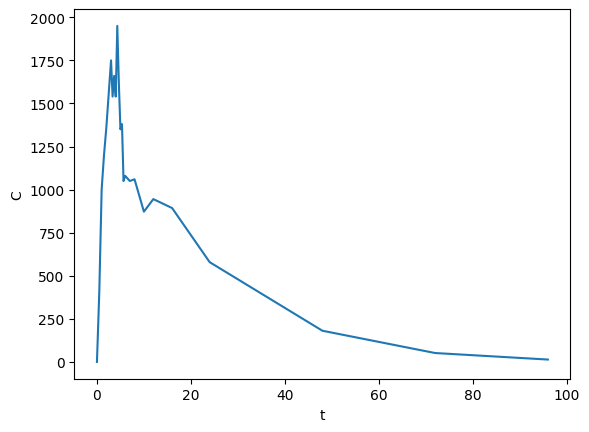
\includegraphics[]{sample.png}

Следует описать основные особеннности имеющихся процессов:

\begin{itemize}
	\item Траектория стартует из нуля.
	\item Данные неоднородны по времени. Хорошо видно, что в самом начале гораздо больше замеров нежели чем ближе к концу траектории.
	\item Единицы измерения по разным осям имеют разные порядки, то есть данные не нормированы.
	\item Сначала концентрация лекарства растёт, затем (с некоторыми оговорками) она убывает.
\end{itemize}

Все дальнейшие рассуждения, связанные с моделями, будут учитывать вышеуказанные особенности.


\newpage

\section{Описание моделей}

\subsection{PBFTPK}

Существуют две различные модификации \textbf{PBFTPK}-модели --- $\textbf{PBFTPK}_0$ и $\textbf{PBFTPK}_1$. Для их описания введём следующие обозначения:

\begin{itemize}
	\item C(t) - \text{концентрация лекарства в крови}
	\item F - \text{биодоступная доля лекарственного средства}
	\item D - \text{введённая доза лекарственного средства}
	\item $V_d$ - \text{объём распределения лекарственного средства}
	\item $k_a$ - \text{коэффициент всасываемости лекарственного средства}
	\item $k_{el}$ - \text{коэффициент выводимости лекарственного средства}
	\item $\tau$ - \text{время абсорбции лекарственного средства}
\end{itemize}

Также условимся называть $C(t)$ при $t < \tau$ ($t \ge \tau$) этапом абсорбции (выведения)

\subsubsection*{$PBFTPK_0$:}

\[
	C(t) = \begin{cases}
		\frac{FD}{\tau} \frac{1}{V_d k_{el}} (1 - e^{-k_{el} t}), t \leq \tau \\
		C(\tau) e^{-k_{el}(t - \tau)}, t > \tau
	\end{cases}
\]

\subsubsection*{$PBFTPK_1$:}

\[
	C(t) = \begin{cases}
		\frac{FD k_a}{V_d (k_a - k_{el})} (e^{-k_{el}t} - e^{-k_a t}), t \leq \tau \\
		C(\tau) e^{-k_{el}(t - \tau)}, t > \tau
	\end{cases}
\]

Недостатком таких моделей является то, что они описывают исключительно процессы с однопиковыми траекториями. Если же траектория процесса может иметь более одного пика, такая модель становится гораздо менее точной. Для исправления этого недостатко можно применить технику ансамблирования моделей.

\subsection{Кусочная модификация PBFTPK}

Модифицируем уже имеющиеся методы оценки параметров модели. Введём параметры $\tau_0$ и $\tau_{max}$ и определим новую модель для случая $\textbf{PBFTPK}_1$ (для случая $\textbf{PBFTPK}_0$ аналогично):

\begin{align*}
	 & C(t) = \begin{cases}
		          0, t \leq \tau_0                                                                    \\
		          \frac{FD k_a}{V_d (k_a - k_{el})} (e^{-k_{el}t} - e^{-k_a t}), \tau_0 < t \leq \tau \\
		          C(\tau) e^{-k_{el}(t - \tau)}, t > \tau
	          \end{cases} \\
	 & \tau_0 < \tau < \tau_{max}                                                                                                                                        \\
\end{align*}

Параметр $\tau_{max}$ является гиперпараметром и задаётся до начала оценки остальных параметров. Для поиска $\tau_0$ и $\tau$ существуют два метода: минимаксный и пиковый. Рассмотрим оба этих метода подробнее.

\subsubsection*{Минимаксный метод}

При использовании этого метода оценки выглядят следующим образом:

\begin{align*}
	\tau = \argmax_{t < \tau_{max}} C(t) \\
	\tau_0 = \argmin_{t < \tau} C(t)
\end{align*}

Этот метод особенно хорошо себя показывает в тех ситуациях, когда траектория имеет ровно одну точку максимума и одну точку минимума, удовлетворяющие необходимым условиям. Если же траектория имеет более сложную форму, более полезным будет второй метод.

\subsubsection*{Пиковый метод}

\begin{align*}
	\tau = max \Argmax_{t < \tau_{max}} C(t) \\
	\tau_0 = max \Argmin_{t < \tau} C(t)
\end{align*}

То есть, вместо поиска условных максимума и минимума функции этот метод выбирает <<максимальные>> точки максимума и минимума соответственно. Основное преимущество этого метода залючается в том, что остатки $r(t) = C(t) - \hat{C}(t)$ будут иметь структуру похожую на исходную траекторию, что пригодится в дальнейшем.

\subsection{EPBFTPK}

Возьмём в качестве базовой модели описанную выше модификацию \textbf{PBFTPK}. Примем $\tau_{max}^1 = +\infty$. Далее одним из перечисленных выше методов оценим параметры $\tau^1$ и $\tau_0^1$: $\hat{\tau}^1$, $\hat{\tau}_0^1$. После поиска параметров \textbf{PBFTPK} получим некую оценку концентрации $\hat{C}_1(t)$. Рассмотрим полученные остатки $r(t) = C(t) - \hat{C}(t)$. Далее тем же методом построим оценку $\hat{C}_2(t)$ для остатков, причём в качестве параметра $\tau_{max}^2$ возьмём полученную ранее оценку $\hat{\tau}^1$. Будем повторять эти шаги до тех пор, пока будет выполняться некий заранее установленный критерий эффективности модели. Итоговая оценка траектории $\hat{C}(t)$ тогда получается следующим образом:

\[
	\hat{C}(t) = \sum_i \hat{C_i}(t)
\]

Полученную модель будем называть \textbf{EPBFTPK} (ensembled PBFTPK).

\subsection{Функции потерь}

Для работы с полученными моделями будем использовать следующую функцию потерь:

\[
	L_{\lambda} = \frac{1}{N} \sum_{i=1}^{N} l_{\lambda}(C, \hat{C}, t_i)
\]

где

\[
	l_{\lambda}(C, \hat{C}, t) = (C(t) - \hat{C}(t)) ^ 2 \cdot \begin{cases}
		1, t \leq \tau \\
		\lambda, t > \tau
	\end{cases}
\]

Здесь и далее будем называть эту функцию $\lambda$ - взвешенной среднеквадратичной функцией потерь ($\textbf{WMSE}_{\lambda}$). Основным достоинством такой функции является возможность регулировать влияние точности на этапе абсорбции на общую точность модели. При $\lambda < 1$ более значительной будет считаться ошибка оценки на этапе абсорбции, при $\lambda > 1$ - на этапе выведения. При $\lambda = 1$ данная функция является обыкновенной квадратичной функцией потерь (\textbf{MSE}).

Стоит заметить, что эта функция в дальнейшем поможет нивелировать недостаток данных, связанный с более редкими измерениями после времени абсорбции.

\subsection{Описание итогового алгоритма}

В итоге, задача оценки траектории с помощью модели сводится к задаче последовательной минимизации:


\[
	L_{\lambda}(r_i, \hat{C}_i, t) \rightarrow \inf_{p \in \Omega}                                          \\
\]
где
\[
	\Omega = \{ (F, D, V_d, k_a, k_{el}) | F \in [0; 1], D \geq 0, V_d \geq 0, k_a \geq 0, k_{el} \geq 0 \} \\
\]
\[
	r_1 = C
\]

Также стоит упомянуть, что данный метод при незначительной модификации может быть использован для предсказания траектории. Для этого нужно будет изменить $l_{\lambda}$ таким образом, что $l_{\lambda} = 0$ при $t > \tau_{max}$, и считать за $\tau_{max}$ время последнего замера концентрации лекарства в крови.

\newpage

\section{Полученные результаты}

На графиках представлены сравнительные результаты работы двух моделей - \textbf{PBFTPK} (сверху) и полчуенной в ходе исследований модели \textbf{EPBFTPK} с взвешенной среднеквадратичной функцией потерь (снизу). Можно заметить, что полученная модель при удачном подброе гиперпараметров (количество моделей в ансамбле, коэффициент $\lambda$, метод оценки абсорбции, и т. д.) оказывается более точной и лучше отражает зависимости в реальных данных. Особенно хорошо это видно в тех случаях, когда после времени абсорбции концентрация убывает не сразу. Стоит отметить, что наименьшую точность модель будет иметь на <<пиках>>, то есть как раз в моменты $\tau_i$.


\begin{center}
	\textbf{Здесь будет таблица со значениями MSE для различных моделей}
\end{center}

\newpage

\begin{minipage}{0.48\linewidth}
	\captionof{figure}{PBFTPK (Пример 1)}
	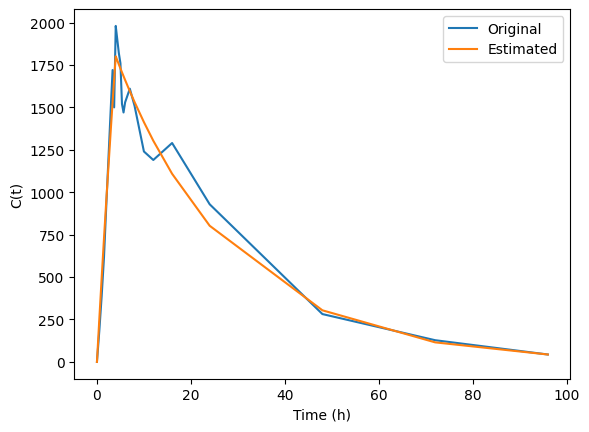
\includegraphics[width=2.0\linewidth]{results/basic_1.png}\newline
	\captionof{figure}{EPBFTPK (Пример 1)}
	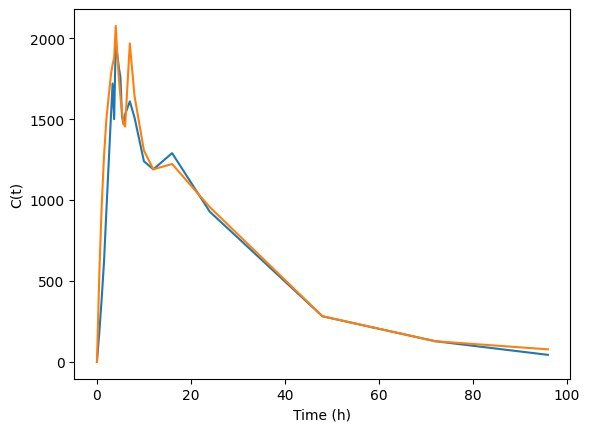
\includegraphics[width=2.0\linewidth]{results/1.jpg}\newline
\end{minipage}

\begin{minipage}{0.48\linewidth}
	\captionof{figure}{PBFTPK (Пример 2)}
	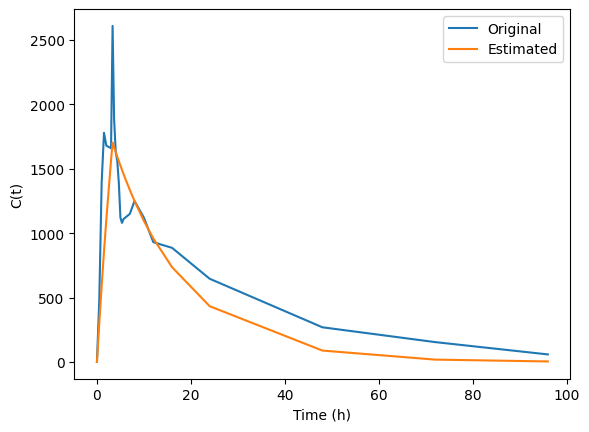
\includegraphics[width=2.0\linewidth]{results/basic_2.png}\newline
	\captionof{figure}{EPBFTPK (Пример 2)}
	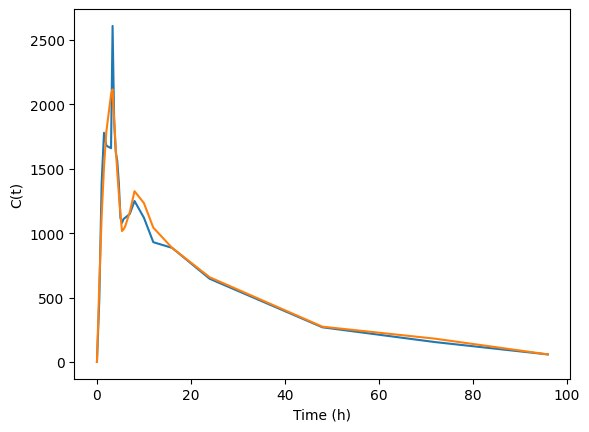
\includegraphics[width=2.0\linewidth]{results/2.jpg}\newline
\end{minipage}


\begin{minipage}{0.48\linewidth}
	\captionof{figure}{PBFTPK (Пример 3)}
	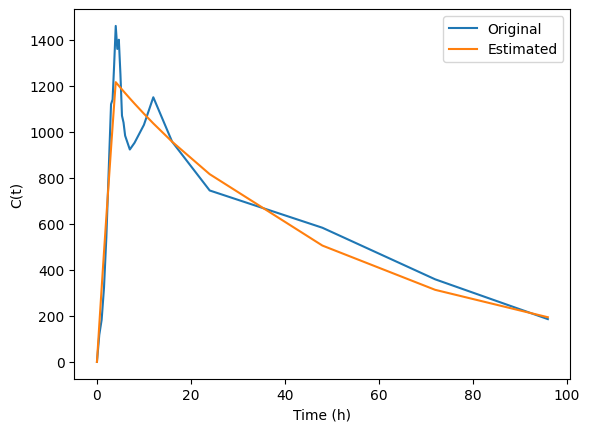
\includegraphics[width=2.0\linewidth]{results/basic_3.png}\newline
	\captionof{figure}{EPBFTPK (Пример 3)}
	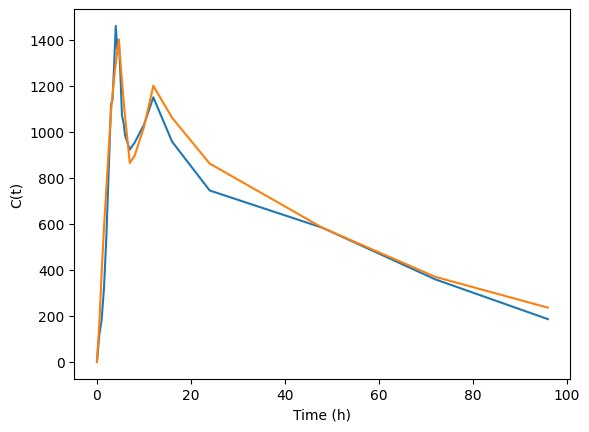
\includegraphics[width=2.0\linewidth]{results/3.jpg}\newline
\end{minipage}

\begin{minipage}{0.48\linewidth}
	\captionof{figure}{PBFTPK (Пример 4)}
	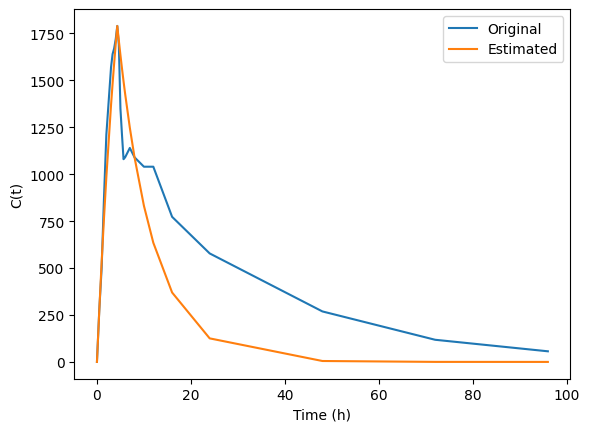
\includegraphics[width=2.0\linewidth]{results/basic_4.png}\newline
	\captionof{figure}{EPBFTPK (Пример 4)}
	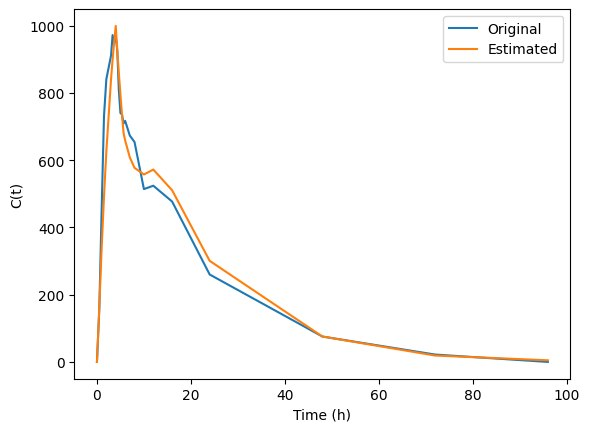
\includegraphics[width=2.0\linewidth]{results/4.jpg}\newline
\end{minipage}

\begin{minipage}{0.48\linewidth}
	\captionof{figure}{PBFTPK (Пример 5)}
	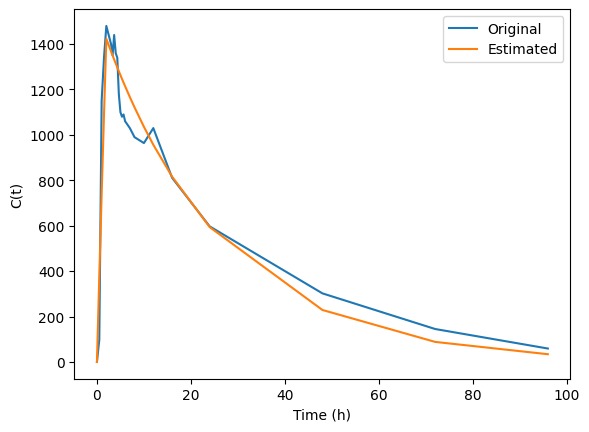
\includegraphics[width=2.0\linewidth]{results/basic_5.png}\newline
	\captionof{figure}{EPBFTPK (Пример 5)}
	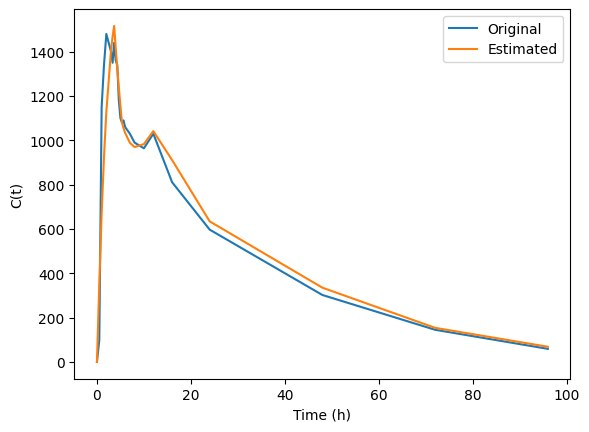
\includegraphics[width=2.0\linewidth]{results/5.jpg}\newline
\end{minipage}

\begin{minipage}{0.48\linewidth}
	\captionof{figure}{PBFTPK (Пример 6)}
	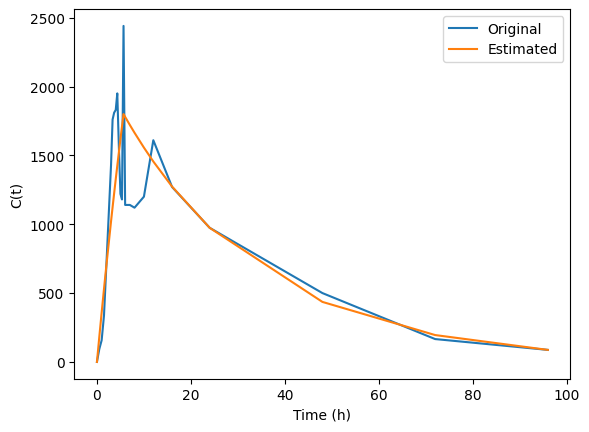
\includegraphics[width=2.0\linewidth]{results/basic_6.png}\newline
	\captionof{figure}{EPBFTPK (Пример 6)}
	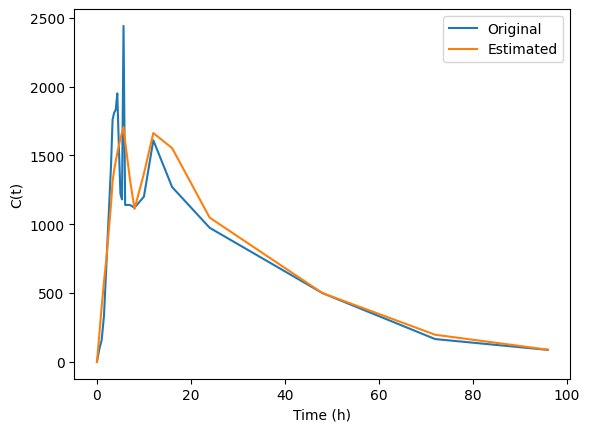
\includegraphics[width=2.0\linewidth]{results/6.jpg}\newline
\end{minipage}

\newpage


\bibliography{refs}

\end{document}
